% !TeX spellcheck = es_ES
\documentclass[12pt, titlepage]{article}
\usepackage[utf8]{inputenc}
\usepackage[spanish]{babel}
\usepackage{float}
\usepackage[letterpaper, margin=2.5cm]{geometry}
\usepackage[nottoc,notlot,notlof]{tocbibind} % Hace que se agregen las referencias al indice
\usepackage{url}
\usepackage{graphicx} 
\usepackage{listings}
\usepackage{color}
\definecolor{dkgreen}{rgb}{0,0.6,0}
\definecolor{gray}{rgb}{0.5,0.5,0.5}
\definecolor{mauve}{RGB}{253,151,31}

\lstset{frame=tb,
    language=Sql,
    aboveskip=3mm,
    belowskip=3mm,
    showstringspaces=false,
    columns=flexible,
    basicstyle={\small\ttfamily},
    numbers=none,
    numberstyle=\tiny\color{gray},
    keywordstyle=\color{blue},
    commentstyle=\color{dkgreen},
    stringstyle=\color{mauve},
    breaklines=true,
    breakatwhitespace=true,
    tabsize=2,
    morekeywords={use}
}

\title{Reporte: Práctica 4}
\author{Carlos Tonatihu Barrera Pérez \\ Profesor: Hernández Contreras Euler \\ Bases de Datos \\ Grupo: 2CM1 }

\begin{document}
\maketitle
\tableofcontents
\section{Marco Teórico}
Esta practica continuo el tema de consultas a una base de datos por lo que es importante señalar lo siguiente.

Las consultas habituales de SQL tien la forma \textbf{select} $A_{1}, A_{2},...,A_{n}$ \textbf{from} $r_{1}, r_{2}, ..., r_{m}$ \textbf{where} $P$.\cite{LIBRO}

Cada $A_{i}$ representa un atributo y cada $r_{j}$ una relación, $P$ es un predicado. SQL forma un producto cartesiano de las relaciones incluidas en la cláusula \textbf{from}, lleva a cabo la selección del álgebra relacional utilizando el predicado de la cláusula \textbf{where} y después proyecta el resultado sobre los atributos de la cláusula \textbf{select}.

Otro concepto del que se hablo en esta practica fueron las operaciones de álgebra relacional, de manera mas especifica se mencionaron tres, \textbf{proyección}, \textbf{producto cartesiano} y \textbf{reunión}.\cite{LIBRO}
\begin{itemize}
	\item La operación \textbf{proyección} es una operación unitaria que devuelve su relación de argumentos, excluyendo algunos argumentos. La proyección se denota por la letra griega mayúscula pi ($\Pi$).
	\item La operación \textbf{producto cartesiano} es denotada por una x ($X$), permite combinar información de cuales quiera dos relaciones.
	\item La operación de \textbf{reunión} es una operación del álgebra relacional extendida, esta operación une dos relaciones que tengan un atributo con el mismo nombre, si no hay ningún nombre en común no se puede realizar. Se denota por el siguiente símbolo $|X|$
\end{itemize}
Existen más operaciones en el álgebra relacional y en el álgebra relacional extendida que serán estudiadas en futuras clases.
\newpage
\section{Desarrollo}
En esta practica se trabajo con la base de datos mostrada en la figura \ref{fig:home} para hacer uso de ella se realizaron los mismos pasos que en practicas anteriores, crear la base, usarla y cargar el script con los datos de la base.
 \begin{figure}[H]
	\begin{center}
		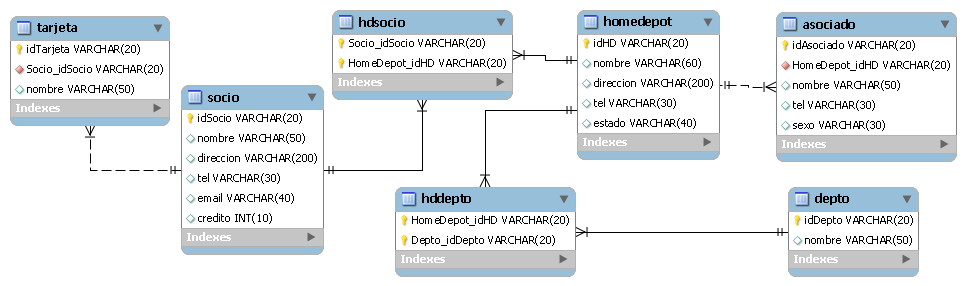
\includegraphics[width=15cm, height=5cm]{img/home.png}
		\caption{Diagrama de la base de datos usada en esta práctica.}
		\label{fig:home}
	\end{center}
\end{figure}
Además, para comenzar a hacer las operaciones necesarias para mostrar su contenido en esta ocasión haciendo uso de más de una tabla y para relacionarlas se utilizo los identificadores de cada relación los cuales se comparaban para obtener el resultado deseado.
 \begin{figure}[H]
	\begin{center}
		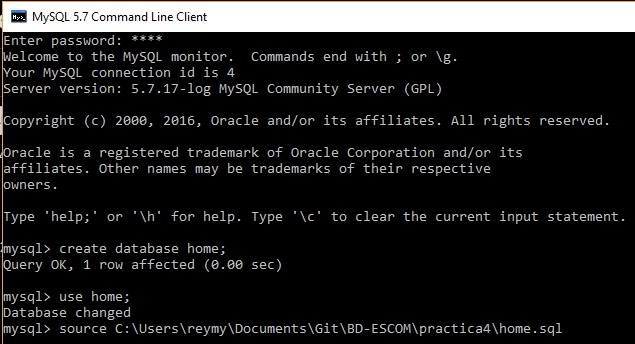
\includegraphics[width=15cm, height=7cm]{img/crear.png}
		\caption{Se crea, usa y se carga la base de datos a usar.}
		\label{fig:home1}
	\end{center}
\end{figure}
Lo primero que se hizo fue listar el nombre de la sucursal y de los empleados asignados mediante el uso de la siguiente instrucción lo cual genero el resultado mostrado en la figura \ref{fig:comando1} en donde se puede ver que la primera ordenación esta basada en homedepot y la segunda en asociado.
 \begin{figure}[H]
	\begin{center}
		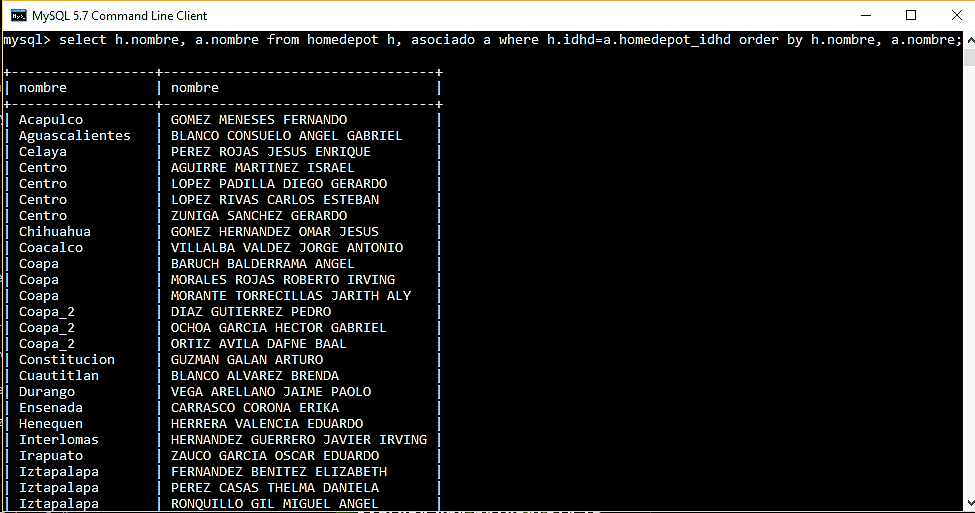
\includegraphics[width=16cm, height=8cm]{img/comando1.png}
		\caption{Primera operación.}
		\label{fig:comando1}
	\end{center}
\end{figure}
Lo siguiente fue mostrar el nombre y correo electrónico de los socios ademas de mostrar la sucursal en donde están dados de alta como se muestra en la figura \ref{fig:comando2}. Es importante mencionar que se usan alias para no tener que escribir el nombre completo de la columna cada vez que se necesita.
 \begin{figure}[H]
	\begin{center}
		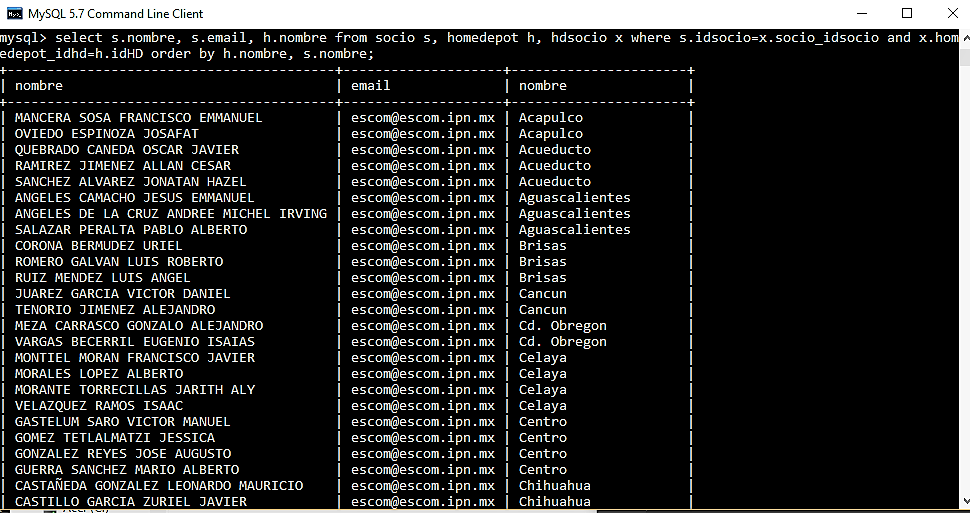
\includegraphics[width=16cm, height=9cm]{img/comando2.png}
		\caption{Operación 2.}
		\label{fig:comando2}
	\end{center}
\end{figure}
Lo siguiente fue mostrar el nombre de los socios, su monto de crédito y la tarjeta que tienen asignada el resultado de esta operación se muestra en la figura \ref{fig:comando3} además de que en lugar de utilizar el nombre de la columna o un alias se utiliza un numero indicando a que columna nos referimos de acuerdo a como están ordenadas entre las palabras reservadas select y from.
 \begin{figure}[H]
	\begin{center}
		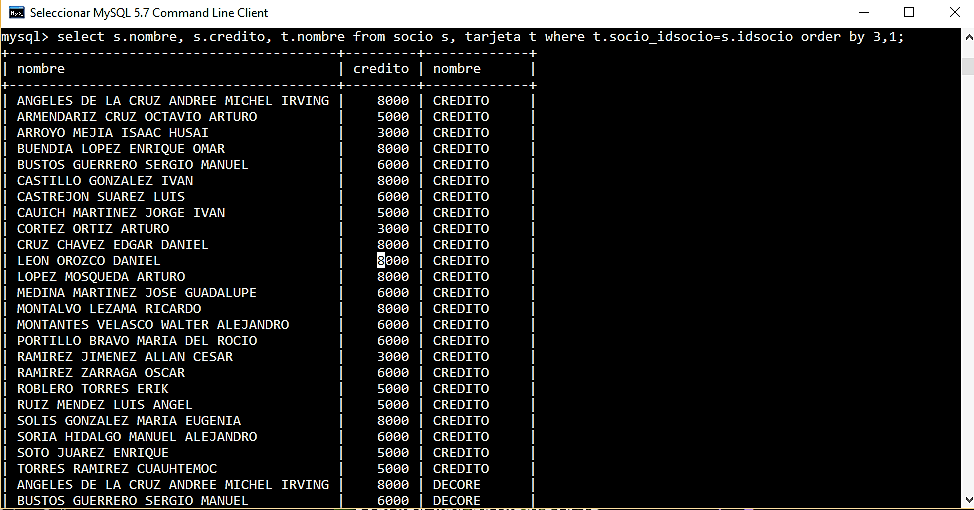
\includegraphics[width=16cm, height=9cm]{img/comando3.png}
		\caption{Algunos socios se repiten debido a que tienen más de un tipo de tarjeta.}
		\label{fig:comando3}
	\end{center}
\end{figure}
Después se imprimió el departamento que tienen las sucursales existentes en el estado de chihuahua lo cual dio como resultado la información mostrada en la imagen \ref{fig:comando4} para realizar esto se utilizo la palabra reservada like.
 \begin{figure}[H]
	\begin{center}
		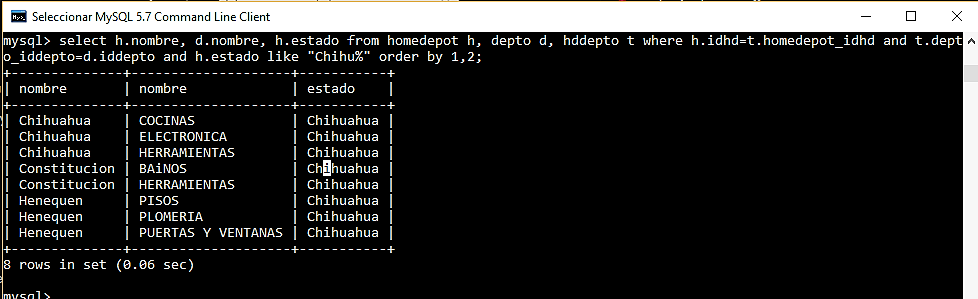
\includegraphics[width=16cm, height=5cm]{img/comando4.png}
		\caption{Las sucursales se repiten debido a que tienen más de un departamentos.}
		\label{fig:comando4}
	\end{center}
\end{figure}
A continuación se mostró el nombre de la sucursal y los empleados que tiene pero solo de las sucursales cuyo código postal es 64830, 53569 y 89360, de nuevo se utilizo la palabra reservada like ya que el código postal se encuentra dentro de la dirección, esto se puede observar en la imagen \ref{fig:comando5}
 \begin{figure}[H]
	\begin{center}
		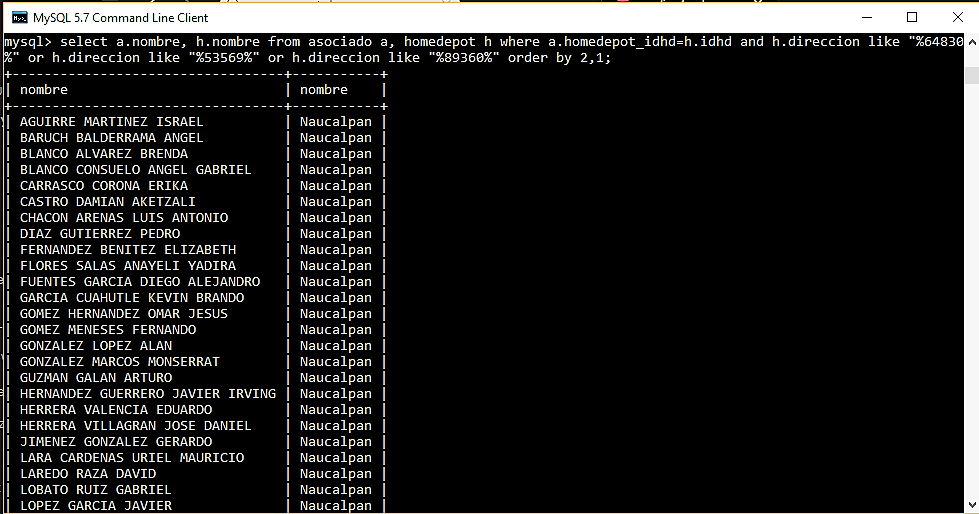
\includegraphics[width=16cm, height=8cm]{img/comando5.png}
		\caption{Una sucursal tiene muchos empleados por lo cual solo se muestra un fragmento de toda la información.}
		\label{fig:comando5}
	\end{center}
\end{figure}
La siguiente operación fue algo confusa debido al orden de ejecución que genera el uso de paréntesis lo cual es importante estudiar a fondo para evitar errores, en este caso se mostró las sucursales en donde se encuentran los socios que se apellidan Gonzáles, al final el resultado fue el que se observa en la figura \ref{fig:comando6}.
 \begin{figure}[H]
	\begin{center}
		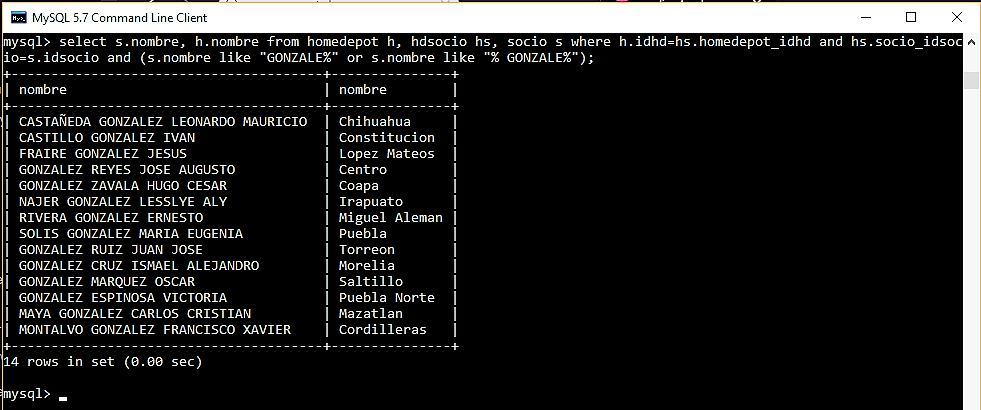
\includegraphics[width=15cm, height=6cm]{img/comando6.png}
		\caption{De no usar los paréntesis la búsqueda tarda más.}
		\label{fig:comando6}
	\end{center}
\end{figure}
La siguiente operación solo mostró cuantos socios se apellidan García para este punto es importante mencionar que lo que se encuentra entre el select y from es una operación de proyección ($\pi$), entre from y where es un producto cartesiano ($x$) y entre where y el resto es una operación reunión ($|x|$).
 \begin{figure}[H]
	\begin{center}
		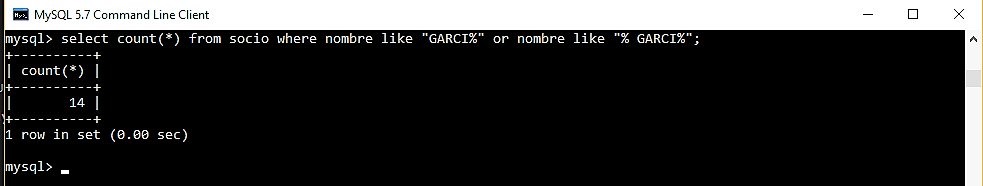
\includegraphics[width=15cm, height=4cm]{img/comando7.png}
		\caption{Solo 7 socios se apellidan García.}
		\label{fig:comando7}
	\end{center}
\end{figure}
Otro punto importante a señalar es que una proyección elimina la duplicidad y hace ordenación Esto se puede observar en las siguientes operaciones en donde la primera no es una proyección (\ref{fig:comando8}) y la segunda y tercera si lo son (\ref{fig:comando9} y \ref{fig:comando10}) en una se utiliza la palabra distinct y en la otra group by.
 \begin{figure}[H]
	\begin{center}
		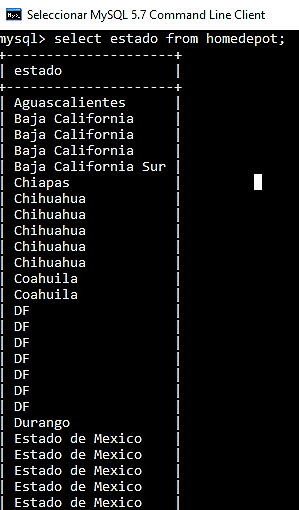
\includegraphics[width=8cm, height=10cm]{img/comando8.png}
		\caption{Esta no es una proyección ya que hay duplicidad y no hay orden.}
		\label{fig:comando8}
	\end{center}
\end{figure}

 \begin{figure}[H]
	\begin{center}
		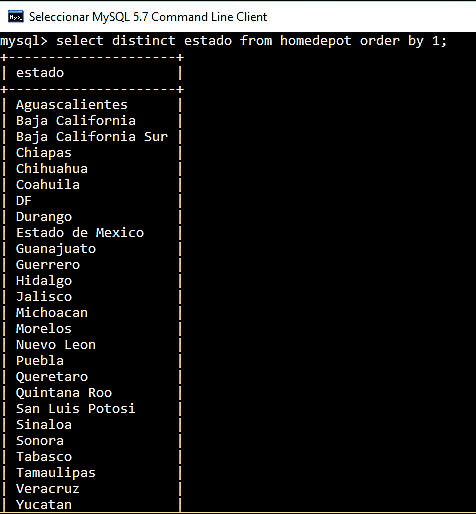
\includegraphics[width=12cm, height=10cm]{img/comando9.png}
		\caption{Operación de proyección usando distinct.}
		\label{fig:comando9}
	\end{center}
\end{figure}
 \begin{figure}[H]
	\begin{center}
		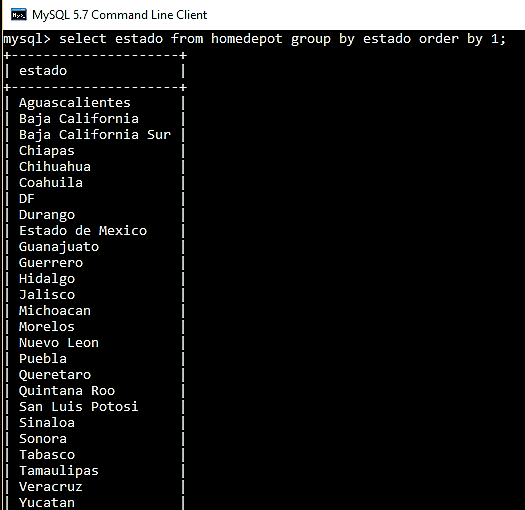
\includegraphics[width=12cm, height=9cm]{img/comando10.png}
		\caption{Usando group by eliminamos la duplicidad y ordenamos.}
		\label{fig:comando10}
	\end{center}
\end{figure}
Lo siguiente fue saber cuantas sucursales existen en los estados, figura \ref{fig:comando11}, de nuevo se utilizo group by.
 \begin{figure}[H]
	\begin{center}
		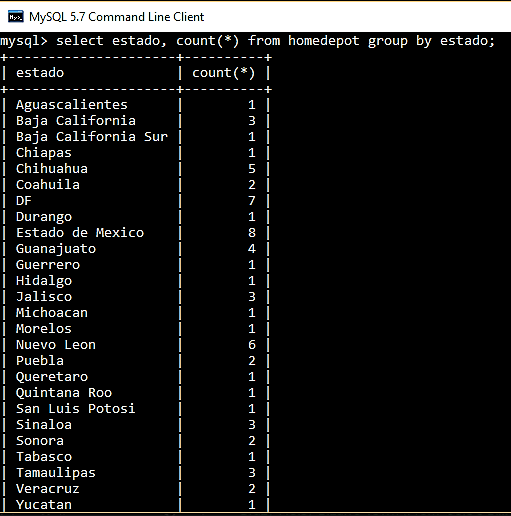
\includegraphics[width=14cm, height=10cm]{img/comando11.png}
		\caption{Se usa group by para evitar duplicidad.}
		\label{fig:comando11}
	\end{center}
\end{figure}
Después, se mostró en cuales sucursales existe el departamento de pisos, el resultado fue el siguiente.
 \begin{figure}[H]
	\begin{center}
		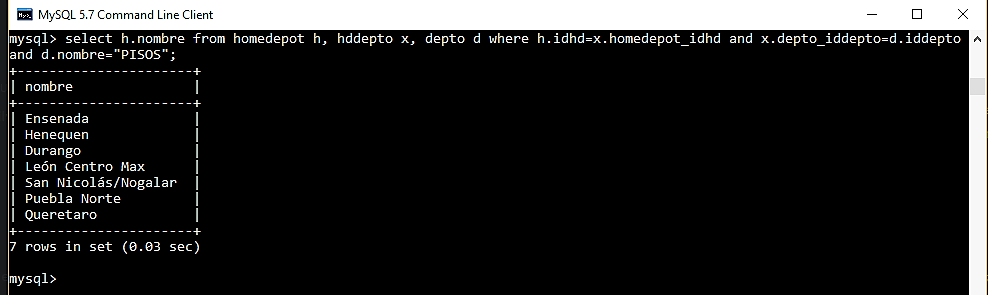
\includegraphics[width=16cm, height=6cm]{img/comando12.png}
		\caption{Las sucursales que tienen el departamento de pisos solo son 7.}
		\label{fig:comando12}
	\end{center}
\end{figure}
Por ultimo, se listo el nombre de los asociados y en que sucursales se ubican al igual que el estado de dichas sucursales.
 \begin{figure}[H]
	\begin{center}
		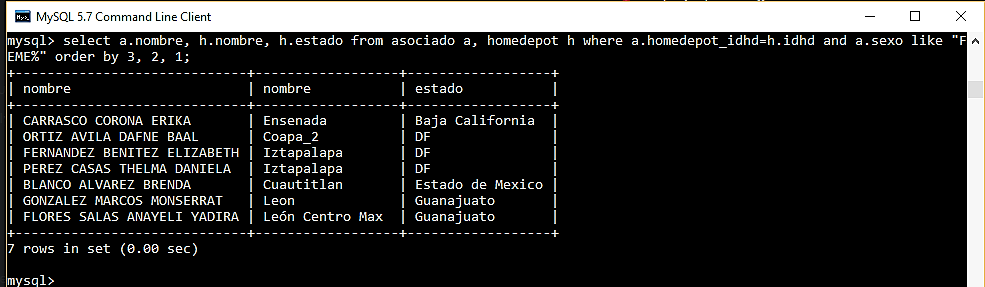
\includegraphics[width=16cm, height=6cm]{img/comando13.png}
		\caption{La primera columna es el asociado, la segunda la sucursal y por ultimo el estado.}
		\label{fig:comando13}
	\end{center}
\end{figure}
\section{Conclusiones}
En esta práctica se continuo con el tema de las consultas a una base de datos que de una forma más especifica es una operación de proyección que hace uso del producto cartesiano y de una operación reunión si es necesario.

Otro punto importe a mencionar es que se pudo observar la gran importancia de los identificadores en las relaciones y el porque se debe de conocer el como utilizarlos de forma correcta para evitar redundancias o problemas a la hora de realizar este tipo de operaciones.

Además, se trabajo con mas de una relación lo cual es importante ya que esto incrementa el nivel de complejidad de las operaciones y por lo tanto se requiere saber que es lo que esta pasando en el fondo y al mismo modo nos ayuda a expandir la funcionalidad de las aplicaciones que realicemos en un futuro y nos presenta un nuevo concepto, los joins que serán estudiados a fondo en futuras practicas.
\bibliography{bibliografia} 
\bibliographystyle{ieeetr}
\end{document}
